% Section 2	- Fundamentals

\section[Fundamentals]{\fontsize{\customSecFontSize}{55}\selectfont Section \arabic{section}}
	% add lof entry - entry before figs in this section
	\addtocontents{lof}{\vspace{\lofSecPreDist}\protect\subsection*{\hspace{\lofSecIndent}Section~\thesection~--~Fundamentals}\vspace{\lofSecPostDist}}
	\addtocontents{lot}{\vspace{\lofSecPreDist}\protect\subsection*{Section~\thesection~--~Fundamentals}\vspace{\lofSecPostDist}}
	\vspace{\customSecPreDist}
	\begin{flushleft}
		{\fontsize{\customSecFontSizeAdd}{\customSecLineDistAdd}\selectfont\bfseries Fundamentals\par}
	\end{flushleft}
	\vspace{\customSecPostDist}
	\label{sec:sec2.fundamentals}

	\vspace{\dropCapSecVertDist}\lettrine{\color{\lettrineDropCapFontColor}{B}}{landit} blandit mauris. \blindtext[1]

	\subsection{Equations}

	Inline usage with \( \partial^2 f / \partial x^2 = 0, \) or spanning over a whole line using
	\[ a^2 + b^2 = c^2. \]
	Equation\,\eqref{eq:sec2.internal_energy} shows an enumerated equation.
	\begin{equation}\label{eq:sec2.internal_energy}
		dU = \underbrace{TdS}_{\delta Q} -pdV + \sum_{i = 1}^{n} \mu_i dN_i + \hdots
	\end{equation}

	\begin{equation}
		\mu_i = \Big( \frac{\partial U}{\partial N_i} \Big)_{S, V, N_{j \neq i}}
	\end{equation}

	Multi-line equation:
	\begin{equation}
	\label{eq:sec2.BV_equation}
		\begin{split}
			\hdots = i_0 \bigg( \frac{C_R(0, t)}{C_R^*}\,\mathrm{e}^{n(1-\alpha)f(E-E^0)}\mathrm{e}^{-nf(1-\alpha)(E_{eq}-E^0)} &- \\
			-\frac{C_O(0, t)}{C_O^*}&\,\mathrm{e}^{-n\alpha f (E- E^0)}\mathrm{e}^{n\alpha f(E_{eq}-E^0)} \bigg)
		\end{split}
	\end{equation}

	Another equation:
	\begin{equation}
		\label{eq:sec2.plane_hagen_poiseuille_flow_profile_avg_vel}
		\overline{v} = \frac{1}{h} \int\limits_{0}^{h} v(z) \, dz = -\frac{1}{h} \int\limits_{0}^{h} \frac{1}{2\mu} \frac{dp}{dx} z\big(h-z\big) \, dz = -\frac{h^2}{12\mu} \frac{dp}{dx}.
	\end{equation}

	\subsection{Tables}
		\textbf{Table 1:}
		% TABLE:	Parameters used for the simulations (Equilibrium potentials, exchange current densities, etc.)
		%
		\newcolumntype{P}[1]{>{\centering\arraybackslash}p{#1}}
		%
		\begin{table}[H]
			\centering
			\caption[Electrochemical cell parameters used for COMSOL Multiphysics simulations]{\textbf{Electrochemical cell parameters used for COMSOL Multiphysics simulations}. Copper was used as a working electrode (WE) and platinum as a counter electrode (CE). Equilibrium potentials \mbox{(eq. pot.)} are referred against the standard hydrogen electrode (SHE) potential.}
			\vspace*{\arryDistTblCap}	%	set distance between table and caption (TOP)
			%								(set in tikz_pgf_settings_and_functions.tex)
			%
			\newcommand{\hcite}{\hspace{-3mm}}	% shift of citations to the left
			%
		%	\begin{tabular}{| P{30mm} | S[table-format=3.4] | L{8mm} | L{62mm} |}	% table formatting
			\begin{tabular}{ P{30mm}  S[table-format=3.4]  L{9mm}  L{62mm} }	% table formatting
				\hline
				% header (first line formatting)
				\noalign{\vskip 0.5mm}	% small vertical whitespace
				\multicolumn{1}{>{\centering\arraybackslash}m{30mm}}{Property}	& \multicolumn{2}{c}{Value}											&	\multicolumn{1}{>{\centering\arraybackslash}m{62mm}}{Description}	\\
				\noalign{\vskip 0.25mm}	% small vertical whitespace
				\hline
				\noalign{\vskip 0.5mm}	% small vertical whitespace
				\( E_{eq, CE} \) [\SI{}{\volt}]						& 1.188		& \hcite\cite{Corrosion_and_prot_eq_pot}							&	\hspace{1cm}Eq. pot. CE against SHE at \celsiustemp{25}				\\
				\( E_{eq, WE} \) [\SI{}{\volt}]						& 0.52		& \hcite\cite{Haynes2010, bard1985standard}							&	\hspace{1cm}Eq. pot. WE against SHE									\\
				\( \sigma \) [\SI{}{\siemens\per\metre}]			& 4.8		& \hcite\cite{Darling1964, hdbkofchem_physics1989, LeeRodkey1966}	&	\hspace{1cm}Electrolyte conductivity								\\
				\( i_{0, CE} \) [\SI{}{\ampere\per\square\metre}]	& 10.0		& \hcite\cite{LandoltBornstein2007, Markovi1997}					&	\hspace{1cm}Exchange current density of CE							\\
				\( i_{0, WE} \) [\SI{}{\ampere\per\square\metre}]	& 240.0		& \hcite\cite{LandoltBornstein2007}									&	\hspace{1cm}Exchange current density of WE							\\
				\noalign{\vskip 0.5mm}	% small vertical whitespace
				\hline
			\end{tabular}
			\label{tab:sec2.e_cell__parameters}
			\vspace{\arryDistTblTextBot}	% 	set distance between table and text (BOTTOM)
			%									(set in tikz_pgf_settings_and_functions.tex)
		\end{table}%

		\textbf{Table 2:}
		% TABLE: evaluation of fit parameters (polynomial regression)
		%
		% Degree	... 	polynomial degree
		% OCV		... 	point of intersection with x-axis (open-circuit voltage)
		% RSS		...		residual sum of squares
		% res min	...		value of the minimum residual
		% res max	...		value of the maximum residual
		%
		% calculated using:	generators/test_cell__potential_variation(time_dep_study__conc_trace)/
		%					/polynomial_fit.py
		%
		\begin{table}[H]
			\centering
			\caption[Parameters of the polynomial regression for the OCV extraction]{\textbf{Parameters of the polynomial regression for the OCV extraction}. Depending on the fitted polynomial degree this table shows the extracted value of the open-circuit voltage (OCV), the residual sum of squares (RSS) as well as the minimum and maximum residual, with the latter two parameters representing the smallest and largest difference between fit values and simulation values.}
			\vspace*{\arryDistTblCap}	%	set distance between table and caption (TOP)
			%								(set in tikz_pgf_settings_and_functions.tex)
			%
			\begin{tabular}[t]{c  c  c  c  c}	% all cells with centred text
				\hline
				% header (first line formatting)
				\noalign{\vskip 0.5mm}	% small vertical whitespace
				Degree	& OCV [\SI{}{\volt}]	& RSS			& Min Residual	& Max Residual	\\
				\noalign{\vskip 0.25mm}	% small vertical whitespace
				\hline
				\noalign{\vskip 0.5mm}	% small vertical whitespace
				3		& -0.6679200			& 2.157771		& -0.47858		& 0.66207		\\
				4		& -0.6678310			& 0.134413		& -0.15257		& 0.13551		\\
				5		& -0.6679710			& 0.014278		& -0.03977		& 0.03924		\\
				6		& -0.6679926			& 0.000694		& -0.02013		& 0.00738		\\
				7		& -0.6679950			& 0.000540		& -0.01786		& 0.00521		\\
				8		& -0.6679950			& 0.000467		& -0.01685		& 0.00590		\\
				9		& -0.6679980			& 0.000380		& -0.01441		& 0.00658		\\
				10		& -0.6679980			& 0.000380		& -0.01409		& 0.00688		\\
				\noalign{\vskip 0.5mm}	% small vertical whitespace
				\hline
			\end{tabular}
			\label{tab:sec2.simple_test_cell_fit_params}
			\vspace{\arryDistTblTextBot}	% 	set distance between table and text (BOTTOM)
			%									(set in tikz_pgf_settings_and_functions.tex)
		\end{table}%

		\textbf{Table 3:}
		% TABLE: 	Dependent variables and their amount depending on the utilised
		%			COMSOL Multiphysics module
		%
		\begin{table}[H]
			\centering
			\caption[Dependent variables depending on the used COMSOL Multiphysics module]{\textbf{Dependent variables depending on the used COMSOL Multiphysics module}. For the three physics modules \textit{laminar flow}, \textit{transport of diluted species} and \textit{electrochemistry} the second column lists the respective dependent variables and the third column the total amount of dependent variables for each module.}
			\vspace*{\arryDistTblCap}	%	set distance between table and caption (TOP)
			%								(set in tikz_pgf_settings_and_functions.tex)
			%
			\newcommand{\toLeft}{\hspace{-2.5mm}}	% shift of citations to the left
			%
			\begin{tabular}{ l r l c c }		% table formatting
				\hline
				% header (first line formatting)
				\noalign{\vskip 0.5mm}	% small vertical whitespace
				\multirow{2}{*}{Physics module}	&	\multicolumn{2}{c}{\multirow{2}{*}{Dependent variables}}	&	Amount of			\\
												&	\multicolumn{2}{c}{}										&	dependent variables	\\
				\noalign{\vskip 0.25mm}	% small vertical whitespace
				\hline
				\noalign{\vskip 0.5mm}	% small vertical whitespace
				\multirow{2}{*}{Laminar flow}	& 	Velocity 			&\toLeft \( \bm{u}(u,v,w) \)			&	\multirow{2}{*}{4}	\\
												& 	Pressure 			&\toLeft \( p\)							&						\\
				\noalign{\vskip 1.0mm}	% small vertical whitespace
				Transport of diluted species	& 	Concentration 		&\toLeft c								&	1					\\
				\noalign{\vskip 1.0mm}	% small vertical whitespace
				Electrochemistry				& 	Liquid potential	&\toLeft \( \phi_l \)					&	1					\\
				\noalign{\vskip 0.5mm}	% small vertical whitespace
				\hline
			\end{tabular}
			\label{tab:sec2.DOFs_depending_on_physics}
			\vspace{\arryDistTblTextBot}	% 	set distance between table and text (BOTTOM)
			%									(set in tikz_pgf_settings_and_functions.tex)
		\end{table}%

	\clearpage
	\subsection{Figures}

		\textbf{Single figure using LaTeX}
		% FIG:	 Example bin for which scattered electrons are collected into
		%
		\begin{figure}[H]%
			\centering
			\subfloat{% FIG:	 Example bin for which scattered electrons are collected into
%
% set viewport and define the variables
\tdplotsetmaincoords{60}{110}

\pgfmathsetmacro{\rvec}{0.8}

\pgfmathsetmacro{\thetavec}{40}
\pgfmathsetmacro{\thetavecTwo}{70}

\pgfmathsetmacro{\phivec}{40}
\pgfmathsetmacro{\phivecTwo}{70}

% create the figure
\begin{tikzpicture}[scale = 6, tdplot_main_coords]

	\coordinate (O) at (0,0,0);

	\draw[thick,->] (0,0,0) -- (0.9,0,0) node[anchor = north east]{$ \textit~{x} ( \theta = 90\,^\circ, \phi = 0\,^\circ)$};
	\draw[thick,->] (0,0,0) -- (0,0.9,0) node[anchor = north west]{$ \textit~{y} ( \theta = 90\,^\circ, \phi = 90\,^\circ)$};
	\draw[thick,->] (0,0,0) -- (0,0,0.9) node[anchor = south]{$ \textit~{z} ( \theta = 0\,^\circ, \phi = 0\,^\circ)$};

	\tdplotsetcoord{P}{\rvec}{\thetavec}{\phivec}
	\tdplotsetcoord{Q}{\rvec}{\thetavec}{\phivecTwo}

	\tdplotsetcoord{P2}{\rvec}{\thetavecTwo}{\phivecTwo}
	\tdplotsetcoord{P3}{\rvec}{\thetavecTwo}{\phivec}

	\draw[-stealth,color = black] (O) -- (P);
	\draw[dashed, color = black] (O) -- (Pxy);
	\draw[dashed, color = black] (P) -- (Pxy);

	\draw[-stealth,color = black] (O) -- (Q);
	\draw[dashed, color = black] (O) -- (Qxy);
	\draw[dashed, color = black] (Q) -- (Qxy);

	\draw[-stealth,color = black] (O) -- (P2);
	\draw[dashed, color = black] (O) -- (P2xy);
	\draw[dashed, color = black] (P2) -- (P2xy);

	\draw[-stealth,color = black] (O) -- (P3);
	\draw[dashed, color = black] (O) -- (P3xy);
	\draw[dashed, color = black] (P3) -- (P3xy);

	\tdplotdrawarc[black, <->, thick]{(O)}{0.3}{0}{\phivec}{anchor = north}{$\phi_1$}
	\tdplotsetthetaplanecoords{\phivec}

	\tdplotdrawarc[tdplot_rotated_coords, <->, thick]{(0,0,0)}{0.5}{0}%
	{\thetavec}{anchor=south west}{$\theta_1$}

	\draw[tdplot_rotated_coords, black] (\rvec,0,0) arc (0:90:\rvec);
	\tdplotsetthetaplanecoords{\phivecTwo}

	\tdplotdrawarc[black, <->, thick]{(O)}{0.6}{0}{\phivecTwo}{anchor=north}{$\phi_2$}
	\tdplotsetthetaplanecoords{\phivecTwo}

	\tdplotdrawarc[tdplot_rotated_coords, <->, thick]{(0,0,0)}{0.6}{0}%
	{\thetavecTwo}{anchor=south west}{$\theta_2$}

	\draw[tdplot_rotated_coords, black] (\rvec,0,0) arc (0:90:\rvec);

	\draw[black] (\rvec,0,0) arc (0:90:\rvec);

	\draw [ultra thick, black] (P) arc (18:92:0.22);
	\draw [ultra thick, black] (Q) arc (-50:-62.5:-3.5);
	\draw [ultra thick, black] (P) arc (-61:-67.7:-7);
	\draw [ultra thick, black] (P3) arc (21.5:90:0.345);

	\begin{scope}[fill = yellow, opacity = 0.4]
		\clip  (P3) arc (21.5:90:0.345) -- (-1.5,0.5) -- (P) arc (-61:-67.7:-7);
		\clip  (Q) arc (-50:-62.5:-3.5) -- (1.0,0.5) -- (P) arc (18:92:0.22);
		\fill (-1,-1) rectangle (1,1.2);
	\end{scope}

	%\draw [ultra thick, red, ->] (0,1) -- (0,0);
	\draw[ultra thick, <-, green] (0,0,0) -- (0,0,0.4) node[anchor = north east]{incident electron beam};

\end{tikzpicture}
}%
			\caption[Example bin: $\theta,\phi \in \lbrack40\,^\circ:70\,^\circ\rbrack$]{Example bin: $\theta,\phi \in \lbrack 40\,^\circ:70\,^\circ\rbrack$.}
			\label{fig:sec2.example_bin_backscatter}
		\end{figure}

		\textbf{Two figures next to each other}

		Generation of figures using functions and from read text files:
		% FIG:	COMSOL simulations: time-dependent study with varying applied potential at WE to determine
		%		the (exact) value of the open-circuit voltage (OCV)
		%
		\begin{figure}[H]%
			\hspace{\initDistDblImg}	% shift both figures to the left
			\hspace{3mm}				% adjust space before figures
			%
			\centering
			%
			% LEFT FIGURE: evolution of concentration in the cell with time
			%
			\subfloat[\label{fig:sec2.simple_test_cell_time_dep_study_OCV_extract_left}]
				{% FIG:	COMSOL simulations: time-dependent study with varying applied potential at WE:
%
% evolution of concentration using a time-dependent study depending on the applied potential
% at the WE. Concentration does not directly start at zero (~10^-13) but has been plotted for simplicity
%
\begin{tikzpicture}[scale = \pScaleImgFactorDblImage, trim axis left, trim axis right]

	%%%%%%%%%%%%%%%%%%%%%%%%%%%%%%%%%%%%%
	%				RAW DATA			%
	%%%%%%%%%%%%%%%%%%%%%%%%%%%%%%%%%%%%%
	% from generators/test_cell__potential_variation(time_dep_study__conc_trace)/slope_extract.ods
	%
	%
	% define slopes here
	%
	% top:
	%
	\newcommand{\slopeTa}{176.1639851269}
	\newcommand{\slopeTaLegend}{-0.80}

	\newcommand{\slopeTb}{87.7510651959}
	\newcommand{\slopeTbLegend}{-0.76}

	\newcommand{\slopeTc}{37.8156703237}
	\newcommand{\slopeTcLegend}{-0.72}

	%
	% bottom:
	%
	\newcommand{\slopeBb}{-18.3708671152}
	\newcommand{\slopeBbLegend}{-0.64}

	\newcommand{\slopeBc}{-54.4576795618}
	\newcommand{\slopeBcLegend}{-0.60}
	%

	% plot variables (since we generate the plot two times for the legends)
	\newcommand{\axisYmin}{-40}
	\newcommand{\axisYmax}{60}
	\newcommand{\axisXmin}{0}
	\newcommand{\axisXmax}{0.5}


	%%%%%%%%%%%%%%%%%%
	%   top legend   %
	%%%%%%%%%%%%%%%%%%
	\begin{axis}[
   					xmin  = \axisXmin,
   					xmax  = \axisXmax,
% 					xtick = {0.0, 0.1,..., 0.50},
					xmajorgrids,
					xlabel = {Time [\SI{}{\second}]},
  					ymin  = \axisYmin,
  					ymax  = \axisYmax,
 					ytick = {-40, -20, 0, 20, 40, 60},
					ylabel = {Concentration [\SI{}{\nano\mol}]},
					ymajorgrids,
					% zerofill the y-axis ticks
					xticklabel style = {
						/pgf/number format/fixed,
						/pgf/number format/fixed zerofill,
						/pgf/number format/precision = 1
					},
 					legend cell align = {right},	% left align the legend entries
					legend pos = north west,
					% legend with two colums
% 					legend columns = 2,
% 					legend style = 	{
% 										/tikz/column 2/.style = 
% 										{
% 											column sep=5pt,
% 										},
% 									}
				]

		% plot the data (top three plots)
		%
		% plot #1
		\addplot[
					loosely dashdotted,
					no marks,
				]
				{x*\slopeTa};	% top -> A
		\addlegendentry{\SI{\slopeTaLegend}{\volt}}



		% plot #2
		\addplot[
					dashdotted,
					no marks,
				]
				{x*\slopeTb};	% top -> B
		\addlegendentry{\SI{\slopeTbLegend}{\volt}}


		% plot #3
		\addplot[
					dotted,
					no marks,
				]
				{x*\slopeTc};	% top -> C
		\addlegendentry{\SI{\slopeTcLegend}{\volt}}
	\end{axis}



	%%%%%%%%%%%%%%%%%
	% bottom legend %
	%%%%%%%%%%%%%%%%%
	\begin{axis}[
   					xmin  = \axisXmin,
   					xmax  = \axisXmax,
					xtick = {0.0, 0.1,..., 0.50},
  					xticklabels = {,,},	% suppress x-ticks (drawn at upper plot)
  					yticklabels = {,,},	% suppress y-ticks (drawn at upper plot)
% 					xmajorgrids,
% 					xlabel = {Time (\SI{}{\second})},
  					ymin  = \axisYmin,
  					ymax  = \axisYmax,
% %   					ytick = {0.1, 0.13,..., 0.22},
% 					ylabel = {Concentration (\SI{}{\micro\Molar})},
% 					ymajorgrids,
% 					% zerofill the y-axis ticks
% 					xticklabel style = {
% 						/pgf/number format/fixed,
% 						/pgf/number format/fixed zerofill,
% 						/pgf/number format/precision = 3
% 					},
 					legend cell align = {right},	% left align the legend entries
					legend pos = south west,
					% legend with two colums
% 					legend columns = 2,
% 					legend style = 	{
% 										/tikz/column 2/.style = 
% 										{
% 											column sep=5pt,
% 										},
% 									}
				]

		% plot the data (bottom three plots)
		%
		% plot #1
		\addplot[
					loosely dashed,
					no marks,
				]
				{x*\slopeBb};	% bottom -> B
		\addlegendentry{\SI{\slopeBbLegend}{\volt}}

		% plot #2
		\addplot[
					dashed,
					no marks,
				]
				{x*\slopeBc};	% bottom -> C
		\addlegendentry{\SI{\slopeBcLegend}{\volt}}

	\end{axis}

\end{tikzpicture}
}%
			%
			\hspace{\distDblImgBetween}
			\hspace{5mm}				% adjust space between figures
			%
			% RIGHT FIGURE: extracted values (slope vs. applied potential) incl. polynomial fit
			%
			\subfloat[\label{fig:sec2.simple_test_cell_time_dep_study_OCV_extract_right}]
				{% FIG:	COMSOL simulations: time-dependent study with varying applied potential at WE:
%
% extracted values: applied potential vs. slope
%
\begin{tikzpicture}[scale = \pScaleImgFactorDblImage*0.95, trim axis left, trim axis right]
	\begin{axis}[
 					xmin  = -0.8,
 					xmax  = -0.6,
   					xtick = {-0.80, -0.76,...,-0.6},
					xmajorgrids,
					xlabel = {Applied potential at WE [\SI{}{\volt}]},
 					ymin  = -50.00,
 					ymax  = 200.00,
%  					ytick = {-40, 0, 40, 80},
					ylabel = {Slope [\SI{}{\nano\mol\per\second}]},
					ymajorgrids,
					% zerofill the y-axis ticks
					xticklabel style = {
						/pgf/number format/fixed,
						/pgf/number format/fixed zerofill,
						/pgf/number format/precision = 2
					},
 					legend cell align = {left},	% left align the legend entries
					legend pos = north east
				]

		% read the data - extracted slope vs. applied potential
		%
		\pgfplotstableread[comment chars = {\%}]
		{2_Sec/generators/test_cell_applied_pot_slope_simulation.txt}
			\avgConcextremelyNormalab;

		% SIMULATION DATA FROM COMSOL
		\addplot [
					color = black,
					mark  = x,
					mark size = 3.0,
					only marks
				]
		table
		[
			x expr=\thisrowno{0},
			y expr=\thisrowno{1},
		] {\avgConcextremelyNormalab};
		\addlegendentry{COMSOL}

		% NUMERICAL FIT - polynom with degree = 10
		%
		% numerical fit:	a_n * x^n + a_(n-1) * x^(n-1) + ... + a_1 * x^1 + a_0
		%
		% add the plot (directly from the .py program)
		\addplot[
					solid,
					samples = \samples,
					no marks,
					domain = -0.80:-0.60
				]
				{-325529.693360*x^10+-573607.060870*x^9+66757.565960*x^8+374041.732600*x^7+-225999.567900*x^6+-171925.347870*x^5+373596.771390*x^4+235387.314490*x^3+-132137.309440*x^2+-138497.155330*x^1+-30445.259211};
				\addlegendentry{Polynomial deg(10)}

	\end{axis}
\end{tikzpicture}
}%
			\caption[Total concentrations with varying applied potential incl. polynomial regression]{\textbf{Total concentrations with varying applied potential inclusive polynomial \mbox{regression}}. The applied potential at the working electrode was varied between \SI{-0.8}{\volt} and \SI{-0.6}{\volt} in steps of \SI{0.01}{\volt} while the total concentration in the cell was tracked. (a) shows a selection of results obtained from these simulations and (b) shows the extracted slopes as well as a fit using a polynomial with tenth degree.}
			\label{fig:sec2.simple_test_cell_time_dep_study_OCV_extract_both}
		\end{figure}

	\clearpage
	\subsection{Pictures}

		% sample holder for the low-temperature measurements
		\begin{figure}[!h]
			\centering
			\subfloat[]{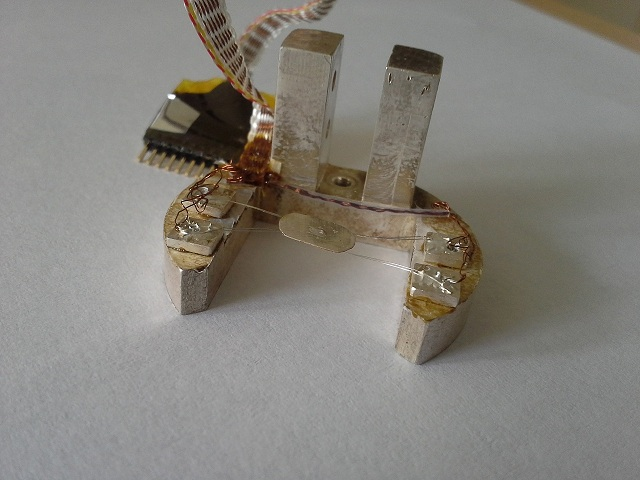
\includegraphics[width=0.48\textwidth]{2_Sec/figures/20170316_112538.jpg}\label{fig:sec2.sample_holder_a}}
			\hfill
			\subfloat[]{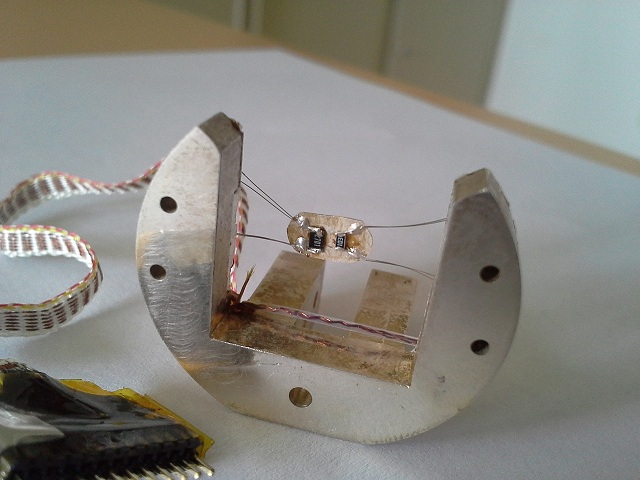
\includegraphics[width=0.48\textwidth]{2_Sec/figures/20170316_112550.jpg}\label{fig:sec2.sample_holder_b}}
			\caption[Sample holder for low-temperature measurements]{Sample holder for the low-temperature measurements. The top side (a) where the grease and sample is placed on a platform made of silver, and the bottom side (b) with the heater (thin film metal resistor 10\,k\(\Omega\)) \mbox{and  thermometer} (RuO2 2.7\,k\(\Omega\)). Please note the four wires (Pt0.9Ir0.1) connecting thermometer and heater each to utilize the 4-point probes method.}
			\label{fig:sec2.sample_holder_both}
		\end{figure}

	\subsection{Indented Source Code}
		%https://docs.scipy.org/doc/scipy/reference/generated/scipy.optimize.leastsq.html
		\verbdef\leastsq{leastsq}
		\verbdef\optimize{scipy.optimize}

		The fit is performed using the function \leastsq\hspace{3px}from the package \optimize\hspace{3px} which takes a function to minimize, initial parameter guesses, the data to fit and some optional arguments as parameter values. For example, the function used to fit \( T_{P_{on}} \) of the two-tau model is given by
\begin{Verbatim}[tabsize=4]
def f(x, K_g, C_s):
	p3 = P_0/K_w+T_0
	alpha = K_w/(2*C_p)+K_g/(2*C_s)+K_g/(2*C_p)
	beta = np.sqrt((C_s*K_w+K_g*C_p+C_s*K_g)**2/(4*C_s**2*C_p**2)- \
		(K_g*K_w)/(C_s*C_p))
	return (P_0/(2*K_w*beta))*((alpha-beta)*np.exp(-x*(alpha+beta))- \
		(alpha+beta)*np.exp(-x*(alpha-beta)))+p3
\end{Verbatim}

	\subsection{Colors}
	% define the colors
	\definecolor{red}{RGB}		{255,	0,		0}
	\definecolor{green}{RGB}	{0,		255,	0}
	\definecolor{blue}{RGB}		{0, 	0, 		255}
	\textcolor{red}{red} \textcolor{green}{green} \textcolor{blue}{blue}
